\documentclass[a4paper, 12pt, titlepage]{article}

\usepackage[utf8]{inputenc}
\usepackage{geometry}
\usepackage{polski}
\usepackage{graphicx} 
\usepackage{float} 
\usepackage{etoolbox,refcount}
\usepackage{multicol}
\usepackage{fancyhdr}
\usepackage{listings}
\usepackage{amsmath}
\usepackage{tabularx}

\newgeometry{left=2.5cm, right=2.5cm, bottom=2.5cm, top=2.5cm}

\lstset{
    language=Matlab,
    basicstyle=\ttfamily,
    keepspaces=true,
    frame=single,
    tabsize=4,
    showspaces=false,
    showstringspaces=false,
    extendedchars=true,
    inputencoding=utf8,
    literate={ó}{{\'o}}1 {ę}{{\k{e}}}1 {ł}{{\l{}}}1 {ż}{{\.z}}1
        {ś}{{\'s}}1 {ć}{{\'c}}1 {ą}{{\k{a}}}1 {ź}{{\'z}}1 {ń}{{\'n}}1
}
\author{Adrian Jałoszewski}
\title{Ćwiczenie 7: Urządzenia wskazujące (,,camera mouse'')}
\date{27 listopada 2017}

\begin{document}
    \maketitle
    \section{Model skóry YCbCr} 
        \begin{figure}[H]
            \centering
            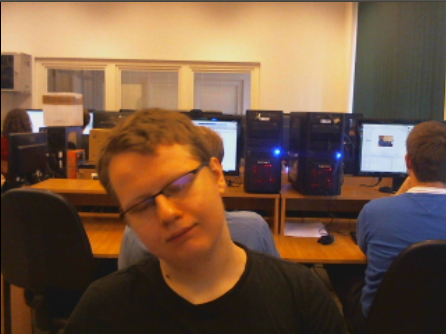
\includegraphics[width=0.8\linewidth]{twarz_kolorowa.png}
            \caption{Twarz kolorowa}
        \end{figure}
        
        \begin{figure}[H]
            \centering
            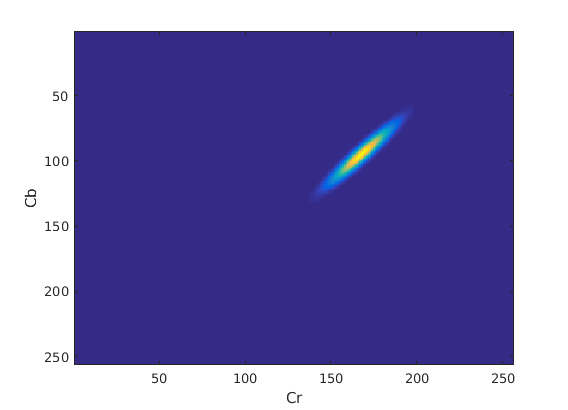
\includegraphics[width=0.8\linewidth]{wizualizacja_modelu_do_sprawozdania.png}
            \caption{Model skóry}
        \end{figure}

        \begin{figure}[H]
            \centering
            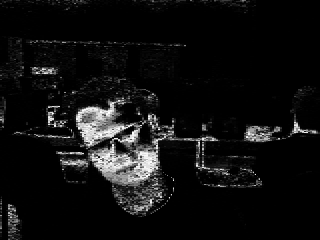
\includegraphics[width=0.8\linewidth]{maj_fejs.png}
            \caption{Obraz prawdopodobieństwa}
        \end{figure}
    \section{Wpływ modelu skóry na rezultaty ćwiczenia}
        Ze względu na otoczenie model koloru skóry ma tutaj bardzo
        duży wpływ na rozpoznanie mojej twarzy. Jej kolor znajduje
        się pomiędzy kolorem biurek oraz ścian w tle. Oprócz tego w
        okolicy siedzą osoby, których szyje można zauważyć na obrazie
        prawdopodobieństwa, podobnie jest z kartonem na lewo od 
        mojej twarzy. Dla takich parametrów jakie zostały ustalone 
        w okolicach jednej trzeciej mojej twarzy jest wykrywanej gorzej
        niż biurka w tle.
    \section{Camshift}
        Algorytm camshift (Continuously Adaptive Meanshift) -- polega na
        nałożeniu pewnego prostokąta na obraz tak aby w środku
        znajdowało się jak najwięcej punktów lub jak w tym przypadku
        suma prawdopodobieństwa w oknie była największa. Okno te jest
        przemiszczane w kierunku środka ciężkości punktów, które się w
        jego obrębie znajdują. Kroki opisane do tej pory dotyczą 
        algorytmu Meanshift. Camshift nastepnie aktualizuje wielkość
        okna o pewien współczynnik $n = \frac{\sqrt{M_{00}}}{8}$
        (zgodnie z OpenCV), a następnie dopasowuje do tak powstałego 
        prostokąta elipsę i określa kierunek jej promieni. Następnie 
        na elipsie opisywany jest prostokąt o bokach prostopadłych do
        kierunków jej promieni.
        \\ \\
        Polepszeniem w stosunku do algorytmu Meanshift jest to, że tak
        ulepszony algorytm lepiej wykrywa obiekty o zmiennej wielkości 
        i o zmiennej rotacji.
    \section{Sterowanie bezwzględne w urządzeniach wskazujących}
        Sterowanie bezwzględne polega na bezpośrednim mapowaniu 
        położenia na położenie kursora. Mapowanie takie ma z zasady
        stały współczynnik CD. Dobrym przykładem takiego urządzenia
        jest tablet (chociaż te też mogą działać na zasadzie sterowania
        względnego). Zwykle w przypadku tego typu urządzeń trudno jest
        zaimplementować akcje wybierania (np. pojedyncze lub podwójne
        kliknięcie).
    \section{Wykres pozycji przed i po skalowaniu, filtracja}
        \begin{figure}[H]
            \centering
            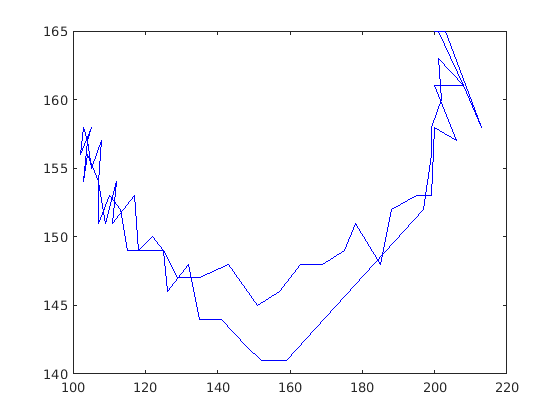
\includegraphics[width=0.8\linewidth]{single_plot.png}
            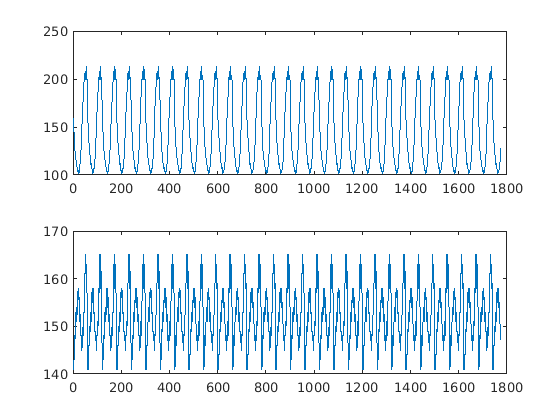
\includegraphics[width=0.8\linewidth]{two_plot.png}
            \caption{Przed filtrowaniem i skalowaniem}
        \end{figure}
        \begin{figure}[H]
            \centering
            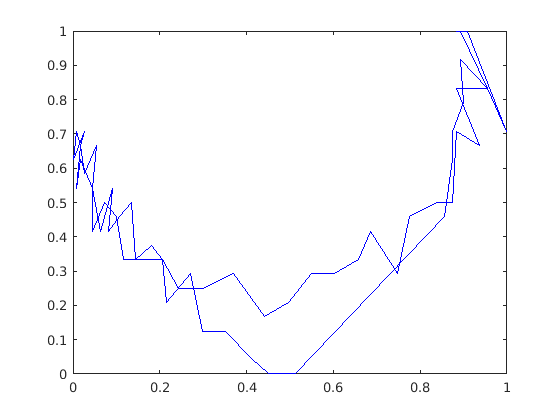
\includegraphics[width=0.8\linewidth]{scaled.png}
            \caption{Po skalowaniu}
        \end{figure}
        Poszczególne parametry:
        \begin{itemize}
            \item[--] ox = 102
            \item[--] oy = 141
            \item[--] sx = 111
            \item[--] sy = 24
            \item[--] N = 10
        \end{itemize}
        Im większa długość filtra tym wynik jest coraz dalszy od 
        wartości skrajnych dla sygnału na którym był kalibrowany
        (musiałoby być co najmniej dziesięć takich samych punktów
        pomiarowych na krawędzi). Dla kalibracji można było 
        zautomatyzować wyszukiwanie \texttt{ox} oraz \texttt{oy}
        przy pomocy znajdowania minimum na osiach.
\begin{lstlisting}
mu1 = getElement(logsout, 'mu2');
mu2 = mu1.Values.Data;

x = mu2(1,1,:); x = x(:);
y = mu2(1,2,:); y = y(:);

x1 = double(x); y1 = double(y);

ox = 102; oy = 141;

x2 = x1 - ox;
y2 = y1 - oy;

sx = (213 - ox); sy = (165 - oy);

x3 = x2 / sx;
y3 = y2 / sy;

\end{lstlisting}
        \begin{figure}[H]
            \centering
            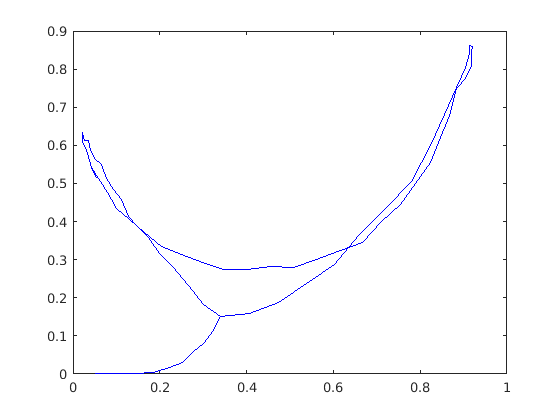
\includegraphics[width=0.8\linewidth]{filtered_2.png}
            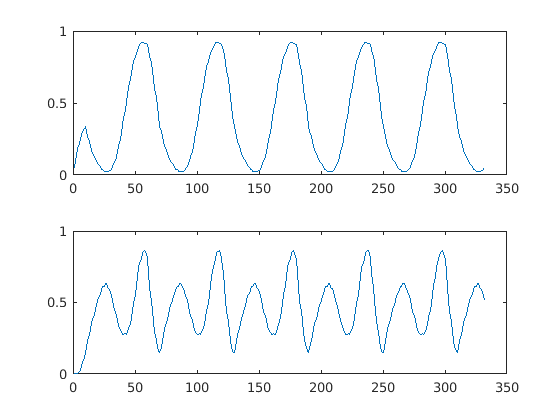
\includegraphics[width=0.8\linewidth]{filtered.png}
            \caption{Po filtrowaniu i skalowaniu}
        \end{figure}
    \section{Lepszy sposób sterowania}
        Nie udało się w czasie trwania ćwiczenia wykonać sterowania ,,on
        line'', jednak już na poziomie analizie danych można wykryć
        pewne problemy z użyciem jako wskaźnika sterowania bezwzględnego.
        W przypadku zbyt dużego oddalenia od kamery można mieć problem z
        koniecznością kalibracji parametrów na nowo, podobnie dzieje
        się w przypadku zbyt małych odległości. Oprócz tego problemem
        jest to, że należy dokonać ruchu o pokaźnych rozmiarach aby 
        dojść od jednej krawędzi do drugiej przy pomocy kursora. 
        Dodatkowo zastosowanie zbyt długiego filtra w celu niwelacji 
        zakłóceń może utrudnić dojście do krawędzi obrazu (obiekt będzie
        powoli do niego zbiegał).
        \\ \\
        Zdecydowanie lepszym rozwiązaniem jest w tym przypadku sterowanie
        względne ze zróżnicowaną funkcją przejścia w zależności od
        prędkości z jaką następuje poruszanie. W ten sposób unika się
        problemu z powolnym zbieganiem do krawędzi oraz innymi problemami
        wynikającymi z dynamiki spowodowanej filtrem.
\end{document}
